\documentclass[12pt,a4paper]{report}
\usepackage[utf8]{inputenc}
\usepackage[portuguese]{babel}
\usepackage{titlesec}
\usepackage{graphicx}
\usepackage{indentfirst}
\usepackage{enumerate}
\usepackage{float}
\usepackage{array}
\usepackage{tikz}
\usepackage{multirow}
\usepackage{multicol}
\usepackage{wrapfig}
\usepackage{geometry}
\usepackage[cache=false]{minted}
\usepackage{pdflscape}
\usepackage[titletoc]{appendix}
\usepackage{hyperref}
\geometry{
 a4paper,
 top=2cm,
 bottom=2cm,
 left=3cm,
 right=3cm
}
\addto\captionsportuguese{
      \renewcommand{\contentsname}
          {Índice}
}
\titleformat{\chapter}{\normalfont\huge}{\thechapter.}{20pt}{\huge}

\begin{document}
\begin{titlepage}
    \center
    {\huge {\bf Universidade do Minho}}\\[0.4cm]
    \vspace{3.0cm}
    \textsc{\huge{Java Factura}}\\[0.5cm]
    \vspace{3.0cm}
    \textsc{\huge{Mestrado Integrado em Engenharia Informática}}\\[0.5cm]
    \vspace{2.0cm}
    \textsc{Programação Orientada a Objectos}\\[0.5cm]
    \textsc{(2º Ano, 2º Semestre, 2017/2018)}\\[0.5cm]
    \vspace{1.5cm}
    \begin{flushleft}
        Grupo 11
        \vspace{1cm}

        A79003 \,\,\,Pedro Mendes Félix da Costa
    \end{flushleft}
        \vspace{1cm}
    \begin{flushright}
        Braga

        Maio 2018
    \end{flushright}

\end{titlepage}

\tableofcontents
\listoffigures

\chapter{Introdução}
    Este trabalho foi realizado no âmbito da unidade curricular programação
    orientada a objectos e teve como objetivo a implementação de um sistema
    similar ao \href{https://faturas.portaldasfinancas.gov.pt}{EFatura}
    aplicando os conceitos lecionados nas aulas.

\chapter{Principais entidades do Sistema}
    \section{Factura}

    \begin{wrapfigure}{r}{5.5cm}
        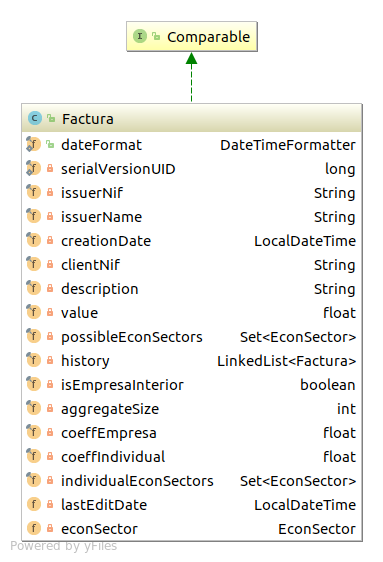
\includegraphics[width=5.5cm]{./images/Factura.png}
        \caption{Diagrama de uma Factura}\label{fig:Factura}
    \end{wrapfigure}

    A classe \textbf{Factura} representa um documento de despesa no sistema.
    Esta por si guarda todas as informações pedidas nos requisitos:
    \begin{multicols}{2}
        \begin{itemize}
            \item NIF do emitente
            \item NIF do cliente
            \item Nome do emitente
            \item Data de criação
            \item Valor da despesa
        \end{itemize}
    \end{multicols}
    Além destes é também guardado um histórico dos estados anteriores da factura
    que é atualizado sempre que o sector de atividade economica desta é
    alterado. Junto a esta é também alterada a data da ultima alteração.

    A alteração do sector economico tem de obedecer a duas restrições para que
    seja executada: 1º Uma factura não pode passar a ser Pendente depois de
    emitida e 2º o sector escolhido tem de ser um dos sectores da empresa que a
    emitiu.

    Para além de todos estes dados uma instancia de \textbf{Factura} guarda
    também alguns dados necessarios para calcular a sua dedução. Estes são:
    \begin{itemize}
        \item Se a empresa que a imitiu é uma empresa do interior
        \item O coeficiente fiscal do emitente
        \item O coeficiente fiscal do cliente
        \item O tamanho do agregado familiar do cliente
        \item Os sectores de actividade para os quais o cliente
            pode deduzir.
    \end{itemize}

\pagebreak

    \section{Sectores de Actividade Económica}
    Todos os sectores economicos extendem a classe \textbf{EconSector} que serve
    apenas para disponibilizar um conjunto de todos os sectores economicos e uma
    metodo de converter o nome do sector na sua repetiva instancia da classe.
    Estas sublcasses por outro lado implementam um padrão \textit{Singleton}, ou
    seja, em qualquer momento exite apenas uma instancia de cada um destes
    objectos em memória. Esta decisão foi tomada porque estes objectos não tem
    estado e como tal são imutaveis, podendo-se assim poupar memória, mas
    sobretudo ter a garantia que as implementações por defeito do
    \mintinline{java}{equals()} e \mintinline{java}{hashcode()} funcionam
    perfeitamente.
    \begin{figure}[h]
        \begin{minted}{java}
public final class Pendente extends EconSector {

    private static final Pendente instance = new Pendente();
    private Pendente(){}
    public static Pendente getInstance(){
        return instance;
    }
    protected Object readResolve(){
        return getInstance();
    }
}
        \end{minted}
        \caption{Implementação \textit{Singleton} da classe \textbf{Pendente}}
        \label{fig:singleton}
    \end{figure}

    Os sectores economicos estão dividos em duas categorias, deduziveis
    e não deduziveis. Esta distinção é feita atravez de uma interface que
    obriga à implementação do metodo \mintinline{java}{deduction()} que calcula
    o valor que é deduzido do valor inicial da despesa.
    \begin{figure}[h]
        \begin{minted}{java}
public interface Deductible {
    float deduction(float value, boolean interior, int numDependants,
                    float coeffEmpresa, float coeffIndividual);
}
        \end{minted}
        \caption{Implementação da interface \textbf{Deductible}}
        \label{fig:deductible}
    \end{figure}

    Os dados necessarios a este calculo são:
    \begin{itemize}
        \item Valor da despesa
        \item Se a factura foi emitida por uma empresa do interior
        \item O numero de dependentes do agregado familiar
        \item O coeficiente fiscal do cliente
        \item O coeficiente fiscal da empresa
    \end{itemize}

    \begin{figure}[h]
        \centering
        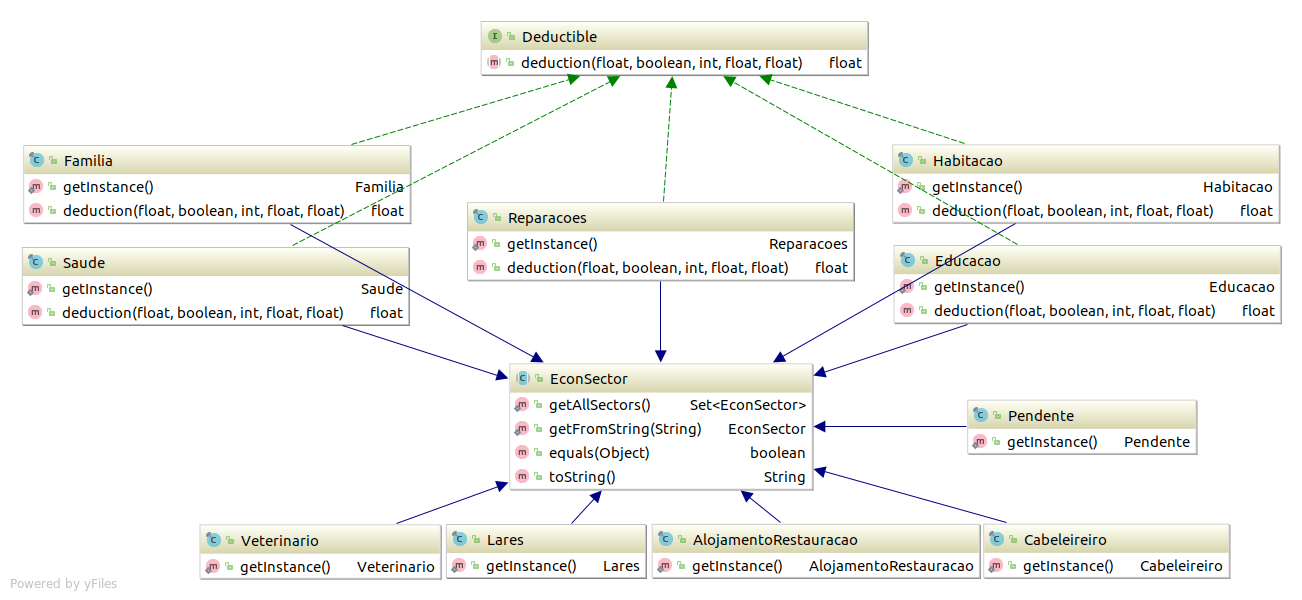
\includegraphics[width=\textwidth]{./images/econSectors.png}
        \caption{Diagrama de classes dos sectores de actividade economica}
        \label{fig:sectors}
    \end{figure}

\pagebreak

    \section{User}
    A interface \textbf{User} é implementada por duas classes, \textbf{Admin} e
    \textbf{Contribuinte}. Esta ultima, sendo um classe abstrata é ainda
    estendida por \textbf{ContribuinteEmpresarial} e
    \textbf{ContribuinteIndividual}.

    Um \textbf{User} tem obrigatoriamente de implementar
    \begin{multicols}{3}
    \begin{itemize}
        \item \mintinline{java}{getNif()}
        \item \mintinline{java}{getName()}
        \item \mintinline{java}{getPassword()}
        \item \mintinline{java}{setPassword()}
        \item \mintinline{java}{clone()}.
    \end{itemize}
    \end{multicols}
    Um \textbf{Admin} implementa apenas a interface, não adicionando mais
    nenhuma funcionalidade, note-se, no entanto, que o nif e nome do admin são
    sempre iguais a "\mintinline{java}{admin}".

    A classe \textbf{Contribuinte} para além de implementar a interface
    guarda também como variaveis o email, morada, coeficiente fiscal, sectores
    de actividade economica, as facturas. Estes ultimos dois atributos são
    vistos de forma diferente dependendo da subclasse que a extende.

    O \textbf{ContribuinteEmpresarial} acrescenta ao \textbf{Contribuinte}
    o \textbf{Conselho}\(\ref{sec:conselho}\) onde reside, este podendo ser
    do interior ou não. Para além disto vê as suas facturas como as vendas que
    realizou os sectores de actividade economica como os possiveis sectores que
    as facturas que emite podem tomar. Estes têm ainda a possibilidade de emitir
    facturas, processo que será explicado em mais detalhe na seccção
     \ref{sec:emissao}.

    O \textbf{ContribuinteIndividual} acrescenta ao \textbf{Contribuinte}
    o agregado familiar e número destes que são dependentes. Este vê as suas
    facturas como as suas despesas e os sectores economicos como o conjunto
    de despesas de onde pode deduzir. Estes têm a capacidade de alterar o
    sector ecnomico das suas facturas.

    \begin{figure}[H]
        \centering
        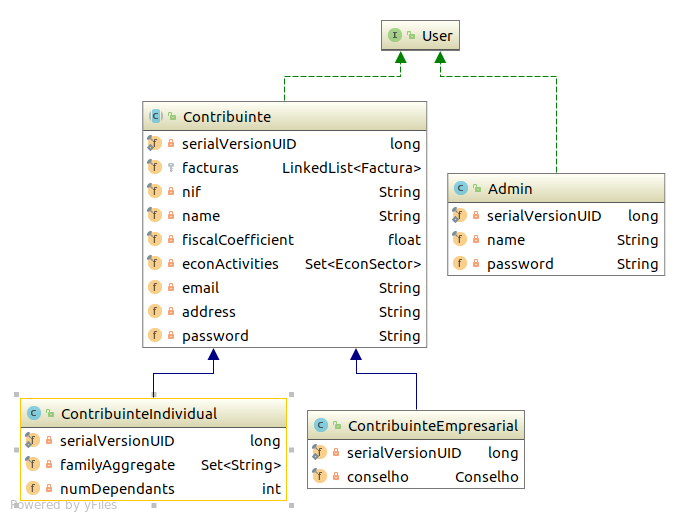
\includegraphics[width=11cm]{./images/UserHierarquy.png}
        \caption{Hierarquia de Classes do \textbf{User}}\label{fig:Hierarquia}
    \end{figure}

\section{Conselhos}
\label{sec:conselho}
    Os conselhos disponiveis são mantidos pela aplicação na forma de um
    \textbf{Enum} que associa a cada um \textit{boolean} a indicar se é um
    conselho do interior ou não. Desta forma simplifica-se bastante o processo
    de distinção das empresa que são ou não do interior. Para além disto, devido
    ao metodo como vai ser utilizado não compromete a extensibilidade do codigo,
    sendo apenas necessario adicionar novas entradas no enum e toda a aplicação
    mantem o um comportamento correto.

    \begin{figure}[h]
        \begin{minted}{java}
public enum Conselho {
    PORTO(false),
    BEJA(true);
    private boolean interior;
    Conselho(boolean interior){
        this.interior = interior;
    }
    public boolean isInterior(){
        return this.interior;
    }
}
        \end{minted}
        \caption{Excerto do enum \textbf{Conselho}}
        \label{fig:conselhos}
    \end{figure}

\chapter{Emissão de Facturas e Calculo de Deduções}

\section{Emissão de Facturas}
\label{sec:emissao}
    Para garantir a consistencia do estado interno da aplicação decidi que
    quando uma factura é emitida tanto o emissor da factura como o cliente
    deviam guardar a mesma instancia do objecto, assim quando o cliente
    eventualmente alterar o sector economico da factura esta alteração é
    automáticamente verificada pela empresa. Para que esta arquitetura não
    pusesse em causa o encapsulamento dos dados apenas instancias de
    \textbf{ContribuinteIndividual} podem alterar facturas. Esta alteração
    é também muito pequena tendo muito pouco impacto para a empresa dados
    os requisitos pedidos.

\section{Calculo de Deduções}
    O a formula de calculo de dedução, como foi referido anterioremente
    \ref{fig:deductible}, a formula de dedução das despesas fica a cargo dos
    sectores economicos, desta forma, para que uma despesa seja deduzivel
    a correspondente factura tera de ser de um sector \textbf{Deductible}
    e de este sector pertencer a lista de sectores a que o cliente esta
    autorizado a deduzir. Um exemplo de uma destas formulas de calculo pode
    ser vista na \textbf{Saude}:
    \begin{figure}[h]
        \begin{minted}{java}
public float deduction(float value, boolean interior, int numDependants,
                       float coeffEmpresa, float coeffIndividual){
    float deduction = 0;
    if(numDependants > 1) deduction += 0.3;
    if(interior) deduction += deduction * 1.5;
    deduction += coeffEmpresa + coeffIndividual;
    return value * deduction;
}
        \end{minted}
        \caption{Formula de calculo implementada para o Sector \textbf{Saude}}
        \label{fig:formulaDeduct}
    \end{figure}

\chapter{Interface Grafica}

    Quando a aplicação inicia o primeiro ecra com que nos deparamos é o de log
    in. Este, se introduzir-mos as credenciais corretas leva-nos a um dos três
    ecras principais.
\begin{figure}[h]
    \centering
    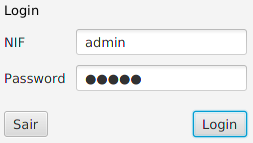
\includegraphics[width=0.5\textwidth]{./images/login.png}
    \caption{Ecra de login}
    \label{fig:login}
\end{figure}

    \section{Admin} %TODO rever
    O ecra do administrador, que pode registar novos contribuintes, individuais
    ou empresariais, ver os 10 contribuintes individuais que gastaram mais
    dinheiro até ao momento ou ver os X contribuintes empresariais que mais
    facturas emitiram junto da quantidade monetaria facturada.
    Este pode ainda alterar a sua password.
\begin{figure}[h]
    \centering
    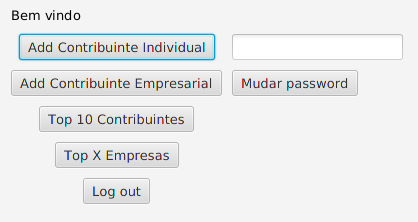
\includegraphics[width=0.5\textwidth]{./images/AdminScreen.png}
    \caption{Ecra do Admin}
    \label{fig:admin}
\end{figure}

\pagebreak

    \section{Contribuinte Individual}
    O ecra do contribuinte individual permite consultar o total deduzido por
    si e pelo seu agregado familiar, consultar as suas facturas ordenadas por
    data ou valor, consultar em detalhe cada factura \(\ref{sec:viewFactura}\)
    e alterar o seu sector economico. Pode ainda consultar o seu perfil onde
    pode alterar o seu email, morada, e password.

\begin{figure}[h]
    \centering
    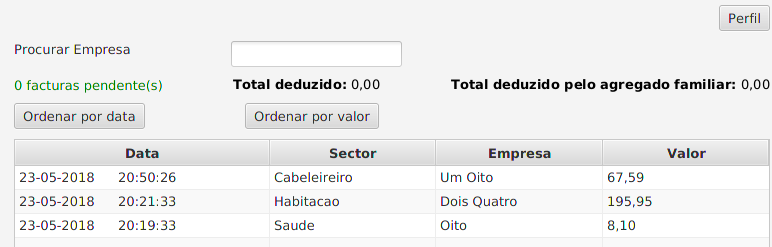
\includegraphics[width=\textwidth]{./images/IndividualScreen.png}
    \caption{Ecra do individual}
    \label{fig:individual}
\end{figure}

    \section{Contribuinte Empresarial}
    O ecra do contribuinte empresarial permite consultar o total facturado
    e facturas emitidas e filtrar ambos por data, para além de as poder ordenar
    como o contribuinte individual pode. Para além disto pode emitir facturas
    novas e ver a lista dos seus clientes. Ao clicar num dos seus clientes pode
    ver todas as facturas deste que foram emitidas por si e, aqui também, pode
    filtrar por data.

\begin{figure}[h]
    \centering
    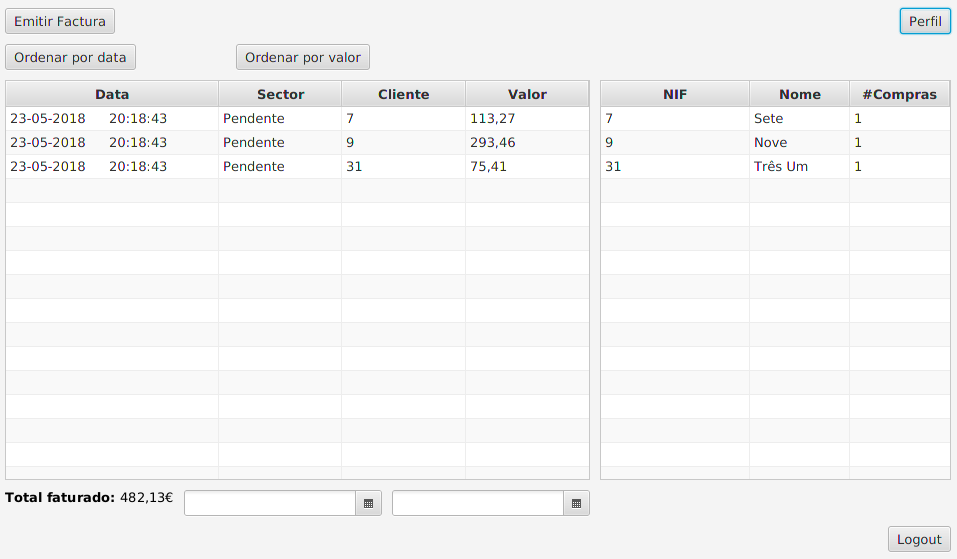
\includegraphics[width=\textwidth]{./images/empresaScreen.png}
    \caption{Ecra do individual}
    \label{fig:individual}
\end{figure}

    \section{Consultar uma Factura}
    \label{sec:viewFactura}
\begin{wrapfigure}{r}{7cm}
    \centering
    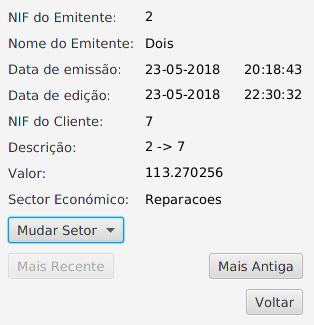
\includegraphics[width=7cm]{./images/facturaView.png}
    \caption{Vista de uma Factura}
    \label{fig:viewFactura}
\end{wrapfigure}
    A consulta de uma factura permite ver todas as alterações que a factura
    sofreu ao longo do tempo e, no caso de o utilizador autenticado ser
    um contribuinte individual, pode também alterar o sector economico desta.

\chapter{Conclusões e Trabalho Futuro}

\end{document}
